\section{Simulation}A series of simulations have been performed to determine the performance of a  $\rm BaF_2$-based or a CsI-based 
calorimeter. The calorimeter geometry is described in the TDR\footnote{Although the geometry has evolved since 
the TDR, the complete set of backgrounds has not been regenerated for the newer designs. Since the background plays 
an important contribution to the resolution, we needed to use the TDR geometry for these studies.}. It is composed 
of two annular disks separated by 700 mm. The disks have inner and outer radii of 351 mm and 660 mm, respectively. 
Both $\rm BaF_2$ and CsI crystals are of hexagonal shape, 33 mm across flats, and 200 mm long. There are a total 
of 1860 crystals. Two readouts are mounted on each crystal to read the scintillation light. Their characteristics 
are detailed below.

Event reconstruction in the calorimeter proceeds in several stages. The interaction of the incident particle with the crystals 
is first simulated by GEANT4, recording the energy, position and time of each step. Each energy deposit is converted into 
scintillation light, taking into account fluctuations of the photo-statistics and non-uniformity in the longitudinal response. 
Corrections from non-linearities in the light production have not been implemented yet. The response of each APD is then simulated, 
including the related electronic noise. A final version of signal digitization and pile-up identification remains to be implemented. 
To simulate these effects, hits within a given time window, depending on the readout characteristics, are grouped together to form 
crystal hits. The crystal hit time is set to the time of the first hit, unless a subsequent hit with at least twice the energy of the 
second most energetic hit is found, in which case the time of that hit is selected.

The crystal hits are then used to form calorimeter clusters. The clustering algorithm starts by taking the crystal hit with the 
largest energy as seed, and adds all simply connected hits within a time window of $\pm 10$ ns and a threshold in energy of either 
3 times the electronic noise or 1 MeV, whichever is larger. The 1 MeV threshold is imposed by the DAQ system limitations. Hits are 
defined as simply connected if they can be reached through a series of adjacent hits. The procedure is repeated until all crystals 
hits are assigned to clusters. Additional low-energy deposits that are disconnected from the main cluster are recovered by dedicated 
algorithms. These fragments are usually produced by the shower, or by low-energy photons emitted by incident particles. 

The energy resolution is estimated by simulating conversion electrons distributed at random in the stopping target foils, 
together with the expected neutron, photon and DIO backgrounds. A few simulations have also been carried out without 
background to assess its impact on the resolution. For CsI crystals, the photon, neutron and DIO backgrounds simulated by Geant4 
(i.e. energy deposits in the crystals) from $\rm BaF_2$ crystals was used. The conversion of energy deposits into scintillation 
light and the subsequent steps are performed using CsI crystals. This approximation should have a limited impact on the results. 
The signal is entirely simulated with CsI crystals. 

The fast scintillation light of $\rm BaF_2$ crystals is read by 9x9 mm$^2$ APD with super-layer treatment and atomic layer deposition 
filter (SL/ALD APD). A UV-extended MPPC with atomic layer deposition filter (ALD MPPC) is also investigated as a possible alternative. 
The SL/ALD APD has a quantum efficiency (QE) of 50\% at 220 nm, following a direct measurement at unity gain, combined with a model 
that RMD uses to track how the QE improves as the device becomes fully depleted under 1800V bias~\cite{docdb-david}. The QE of 
UV-extended MPPC at 220 nm is approximately 20\%~. The readout selected for CsI crystals is a UV-extended SPL MPPC, with a 
QE at the level of 40\% at 310 nm~\cite{docdb5166}. The electronic noise has been estimated to be 300 keV/APD for $\rm BaF_2$ crystals, 
extrapolated on measurements from LYSO, and 100 keV/MPPC for CsI crystals~\cite{docdb5405}.  

The number of photo-electrons per MeV ($N_{p.e./ MeV}$) for $\rm BaF_2$ is derived following a measurement of 160 p.e./MeV for the fast 
component (220 nm) using a photo-multiplier having a 30\% quantum efficiency and a surface of 950 mm$^2$ with grease and 8 layers teflon 
wrapping~\cite{docdb5716}. A number of 30 photo-electrons per MeV for CsI crystal has been measured using the UV-extended SPL 
MPPC~\cite{docdb5166}. The longitudinal response uniformity (LRU) is modeled by a single linear component describing the level of 
non-uniformity at the end of the crystal w.r.t. its center. A nominal value of 5\% is used.
 
Several simulations are performed for the combinations of crystals and sensors described above. In addition, we study the sensitivity of 
the results to the integration time, light yield, electronic noise and longitudinal response uniformity for $\rm BaF_2$ crystals with 
SL/ALD APD and CsI crystals with MPPC. The complete set of parameters are summarized in Table~\ref{sim:tab::BaF2} and \ref{sim:tab::Csi}. 
We also perform a few simulations without background to assess its effect on the resolution. 

\begin{table}[htb]
\begin{center}
\begin{tabular}{|c|c|c|c|c|c|c|}\hline
Sim.   & Readout      & Integration & $N_{p.e./ MeV}$ & Noise & LRU & Other \\ 
number & type         & time (ns)   &   per readout   & (keV) & (\%)& \\\hline
1      & SL/ALD APD   &  60         & 23              & 300   &  5  & default \\
2      & SL/ALD APD   &  60         & 15              & 450   &  5  & \\
3      & SL/ALD APD   &  60         & 10              & 700   &  5  & \\
4      & SL/ALD APD   &  60         &  8              & 900   &  5  & \\
5      & SL/ALD APD   &  60         & 23              & 200   &  5  & \\
6      & SL/ALD APD   &  60         & 23              & 400   &  5  & \\
7      & SL/ALD APD   &  60         & 23              &1000   &  5  & \\
8      & SL/ALD APD   &  60         & 23              &2000   &  5  & \\
9      & SL/ALD APD   &  60         & 23              & 300   & 15  & \\
10     & SL/ALD APD   &  60         & 23              & 300   & 25  & \\
11     & SL/ALD APD   &  60         & 23              & 300   &  5  & Bkg x2 \\
12     & SL/ALD APD   &  60         & 23              & 300   &  5  & Bkg x4 \\
13     & SL/ALD APD   &  60         & 23              & 300   &  5  & $E_{cut,cluster} = 1.5$  \\
14     & SL/ALD APD   &  60         & 23              & 300   &  5  & $E_{cut,cluster} = 2.0$  \\
100    & ALD VUV MPPC & 150         & 16              & 200   &  5  &        \\ \hline
200    & SL/ALD APD   &  60         & 23              & 300   &  5  & No Bkg \\ 
201    & SL/ALD APD   &  60         & 23              & 300   &  5  & No Bkg, $E_{cut,cluster} = 1.5$ \\ 
202    & SL/ALD APD   &  60         & 23              & 300   &  5  & No Bkg, $E_{cut,cluster} = 2.0$ \\ \hline
\end{tabular}
\end{center}
\caption{Parameters of the simulations performed for BaF$_2$ crystals with background. The number of 
p.e./MeV and the noise are given per readout. Two readouts are mounted on each crystal. The variable 
$E_{cut,cluster}$ denotes minimum energy required for a hit to be included in the cluster (see related 
discussion on cluster reconstruction above).}
\label{sim:tab::BaF2}
\end{table}   

\begin{table}[htb]
\begin{center}
\begin{tabular}{|l|l|c|c|c|c|c|}\hline
Sim.   & Readout      & Integration & $N_{p.e./ MeV}$ & Noise & LRU & Other \\ 
number & type         & time (ns)   &  per readout    & (keV) &     & \\ \hline
1     & MPPC          & 150         &  30             & 100   &  5  &  default \\
2     & MPPC          & 150         &  20             & 150   &  5  &       \\
3     & MPPC          & 150         &  15             & 200   &  5  &       \\
4     & MPPC          & 150         &  10             & 300   &  5  &       \\
5     & MPPC          & 150         &  30             & 100   & 15  &       \\
6     & MPPC          & 150         &  30             & 100   & 25  &       \\
7     & MPPC          &  60         &  30             & 100   &  5  & $\rm T_{int}$ of BaF$_2$ \\
8     & MPPC          & 150         &  30             & 100   &  5  & Bkg x2 \\
9     & MPPC          & 150         &  30             & 100   &  5  & Bkg x4 \\ 
10    & MPPC          & 150         &  30             & 100   &  5  & $E_{cut,cluster} = 1.5$ MeV \\ 
11    & MPPC          & 150         &  30             & 100   &  5  & $E_{cut,cluster} = 2.0$ MeV \\ \hline
200   & MPPC          & 150         &  30             & 100   &  5  & No bkg \\ 
201   & MPPC          & 150         &  30             & 100   &  5  & No bkg, $E_{cut,cluster} = 1.5$ \\ 
202   & MPPC          & 150         &  30             & 100   &  5  & No bkg, $E_{cut,cluster} = 2.0$ \\ \hline
\end{tabular}
\end{center}
\caption{Parameters of the simulations performed for CsI crystals with background. The number of p.e./MeV and the 
noise are given for a single readout. Two readouts are used per crystal. The variable $E_{cut,cluster}$ denotes 
minimum energy required for a hit to be included in the cluster (see discussion above).}
\label{sim:tab::Csi}
\end{table}   

The distribution of the difference between the reconstructed cluster energy and the true signal electron energy, $\Delta E = E_{clu}-E_{trk}$, 
are shown in Figure~\ref{sim::fig::fits} for a few simulations. This variable accounts for the energy lost by the electron before hitting 
the calorimeter. The high-side tail is due to background pile-up with the cluster. An unbinned likelihood fit to the data with a Crystal 
Ball function (Gaussian function with a power-law tail) is performed to extract the resolution. The core resolution (Gaussian component) 
and the FWHM/2.35 are reported in Table~\ref{sim:results1} and \ref{sim:results2}. The quoted uncertainties are only statistical, and 
systematic uncertainties due to the choice of the fit model could be as large as the statistical components for some configurations. 

The core resolution and FHWM/2.35 for the $\rm BaF_2$ crystals with SL/ALD APD (CsI crystal with MPPC) are $3.6 \pm 0.2$ MeV ($ 4.2 \pm 0.3$ MeV) 
and $4.4\pm 0.3$ MeV ($5.7 \pm 0.3$ MeV), respectively. The comparison of the two $\Delta E$ spectra are shown in Figure~\ref{sim::fig::fitsBaCsi}. 
The resolution for CsI is about 10\% larger, mostly due to the effect of additional noise integrated over a longer time window compared to 
barium fluoride. Improved treatment of the waveform digitization and hit extraction should partially alleviate this difference. We also note 
that the different readouts for $\rm BaF_2$ crystals yield fairly similar results; the SL/ALD APD performing slightly better than the 
UV-extended ALD MPPC.

The dependence on the light yield, longitudinal response uniformity and readout noise are displayed in Figure~\ref{sim::fig::param} 
and \ref{sim::fig::param2}. As expected, the resolution degrades with the decrease of the light yield, the longitudinal response uniformity, 
or the electronic noise. The resolutions remains in an acceptable range, except in the of large APD noise (larger than 1 MeV). In this 
case, the CsI based calorimeter seems to be a better alternative. 

The impact of the level of background is shown in Figure~\ref{sim::fig::bkg}. Increasing the background by a factor of four results in a $\sim30\%$ 
($\sim 50\%$) increase of the resolution for barium fluoride (cesium iodine) crystals with our current version of hit digitization. Improved treatment 
of the pile-up will certainly lead to better results. The effect of varying the threshold in energy in the clustering algorithm from 1.0 MeV to 2.0 MeV 
is illustrated in Figure~\ref{sim::fig::fitsNobkg2}, for simulations with and without background. Once again, the impact on the resolution is small.

Finally, we show the signal acceptance in Figure~\ref{sim::fig::effi}, defined as the number of events having a reconstructed track and an electromagnetic 
cluster above a given energy threshold normalized to the number of events containing a reconstructed track. Since the absolute value of energy spectra are 
not properly calibrated yet, the peak of each cluster energy distribution is arbitrarily set to 100 MeV. An efficiency slightly above to 90\% (65\%) is 
observed for cluster energies above 60 MeV (90 MeV). The differences in efficiency between $\rm BaF_2$ and CsI are partly due to the crude hit extraction 
procedure.

\begin{table}[htb]
\begin{center}
\begin{tabular}{|c|c|c|c|c|c|c|c|}\hline
Sim.       & Readout      & $\rm T_{int}$ & $N_{p.e./ MeV}$ & Noise   & $\sigma$  & FWHM/2.35 & other \\
number     &              & (ns)          &                 & (keV)   &  (MeV)    & (MeV)     & \\\hline         
1          & SL/ALD APD   & 60            & 23              & 300     & $ 3.6 \pm 0.2 $  & $ 4.4 \pm 0.2 $ &default\\
2          & SL/ALD APD   & 60            & 15              & 450     & $ 4.1 \pm 0.2 $  & $ 4.4 \pm 0.2 $ &\\
3          & SL/ALD APD   & 60            & 10              & 700     & $ 4.4 \pm 0.4 $  & $ 5.1 \pm 0.3 $ &\\
4          & SL/ALD APD   & 60            &  8              & 900     & $ 5.3 \pm 0.3 $  & $ 5.7 \pm 0.2 $ &\\
5          & SL/ALD APD   & 60            & 23              & 200     & $ 3.3 \pm 0.2 $  & $ 4.0 \pm 0.2 $ &\\
6          & SL/ALD APD   & 60            & 23              & 400     & $ 4.0 \pm 0.2 $  & $ 4.6 \pm 0.2 $ &\\
7          & SL/ALD APD   & 60            & 23              &1000     & $ 5.9 \pm 0.4 $  & $ 6.9 \pm 0.3 $ & \\ 
8          & SL/ALD APD   & 60            & 23              &2000     & $ 7.6 \pm 1.0 $  & $ 8.8 \pm 0.5 $ &\\ 
9          & SL/ALD APD   & 60            & 23              & 300     & $ 3.9 \pm 0.2 $  & $ 4.7 \pm 0.2 $ & 15\% LRU\\
10         & SL/ALD APD   & 60            & 23              & 300     & $ 4.3 \pm 0.4 $  & $ 5.6 \pm 0.2 $ & 25\% LRU\\
11         & SL/ALD APD   & 60            & 23              & 300     & $ 4.2 \pm 0.2 $  & $ 4.9 \pm 0.2 $ & Bkg x2\\
12         & SL/ALD APD   & 60            & 23              & 300     & $ 5.5 \pm 0.3 $  & $ 5.8 \pm 0.3 $ & Bkg x4\\ 
13         & SL/ALD APD   & 60            & 23              & 300     & $ 4.0 \pm 0.2 $  & $ 4.7 \pm 0.2 $ & $E_{cut,cluster} = 1.5$  \\
14         & SL/ALD APD   & 60            & 23              & 300     & $ 4.0 \pm 0.2 $  & $ 4.6 \pm 0.2 $ & $E_{cut,cluster} = 2.0$  \\
100        & ALD VUV MPPC & 150           & 16              & 200     & $ 4.2 \pm 0.4 $  & $ 5.2 \pm 0.3 $ & \\\hline
200        & SL/ALD APD   & 60            & 23              & 300     & $ 2.2 \pm 0.1 $  & $ 2.9 \pm 0.1 $ & No Bkg \\ 
201        & SL/ALD APD   & 60            & 23              & 300     & $ 2.8 \pm 0.1 $  & $ 3.2 \pm 0.1 $ & No Bkg, $E_{cut,cluster} = 1.5$\\
202        & SL/ALD APD   & 60            & 23              & 300     & $ 2.7 \pm 0.1 $  & $ 3.4 \pm 0.1 $ & No Bkg, $E_{cut,cluster} = 2.0$\\ \hline
\end{tabular}
\end{center}
\caption{The core resolution ($\sigma$) and the FWHM/2.35 extracted from the fits to the different simulations for BaF$_2$ 
crystals. The number of p.e./MeV and the noise are given per readout.}
\label{sim:results1}
\end{table}   

\begin{table}[htb]
\begin{center}
\begin{tabular}{|c|c|c|c|c|c|c|c|}\hline
Sim.       & Readout      & $\rm T_{int}$ & $N_{p.e./ MeV}$ & Noise & core resolution  & FWHM/2.35 & other\\
number     & type         &  (ns)         &                 & (keV) & $\sigma$ (MeV)   & (MeV)     &      \\\hline
1          & MPPC         & 150           &  30             & 100    & $ 4.2 \pm 0.3 $  & $ 5.7 \pm 0.3 $ & default\\
2          & MPPC         & 150           &  20             & 150    & $ 4.1 \pm 0.4 $  & $ 6.0 \pm 0.3 $ & \\
3          & MPPC         & 150           &  15             & 200    & $ 4.3 \pm 0.4 $  & $ 5.9 \pm 0.2 $ & \\
4          & MPPC         & 150           &  10             & 300    & $ 5.6 \pm 0.4 $  & $ 6.4 \pm 0.4 $ & \\
5          & MPPC         & 150           &  30             & 100    & $ 5.1 \pm 0.4 $  & $ 6.6 \pm 0.3 $ & 15\% LRU \\
6          & MPPC         & 150           &  30             & 100    & $ 5.2 \pm 0.5 $  & $ 6.4 \pm 0.4 $ & 25\% LRU \\
7          & MPPC         &  60           &  30             & 100    & $ 3.7 \pm 0.3 $  & $ 4.5 \pm 0.2 $ & $\rm T_{int}$ of BaF$_2$ \\ 
8          & MPPC         & 150           &  30             & 100    & $ 5.1 \pm 0.5 $  & $ 6.6 \pm 0.3 $ & Bkg x2 \\
9          & MPPC         & 150           &  30             & 100    & $ 7.6 \pm 0.7 $  & $ 8.9 \pm 0.6 $ & Bkg x4 \\
10         & MPPC         & 150           &  30             & 100    & $ 4.6 \pm 0.4 $  & $ 6.3 \pm 0.3 $ & $E_{cut,cluster} = 1.5$ \\
11         & MPPC         & 150           &  30             & 100    & $ 4.4 \pm 0.4 $  & $ 6.0 \pm 0.3 $ & $E_{cut,cluster} = 2.0$ \\\hline
200        & MPPC         &  60           &  30             & 100    & $ 2.5 \pm 0.1 $  & $ 3.5 \pm 0.1 $ & No Bkg \\ 
201        & MPPC         &  60           &  30             & 100    & $ 2.9 \pm 0.1 $  & $ 3.7 \pm 0.1 $ & No Bkg, $E_{cut,cluster} = 1.5$ \\ 
202        & MPPC         &  60           &  30             & 100    & $ 3.4 \pm 0.1 $  & $ 4.0 \pm 0.1 $ & No Bkg, $E_{cut,cluster} = 2.0$ \\ \hline
\end{tabular}
\end{center}
\caption{The core resolution ($\sigma$) and the FWHM/2.35 extracted from the fits to the different simulations for CsI 
crystals. The number of p.e./MeV and the noise are given per readout.}
\label{sim:results2}
\end{table}   



\begin{figure}[htb]
\begin{center}
   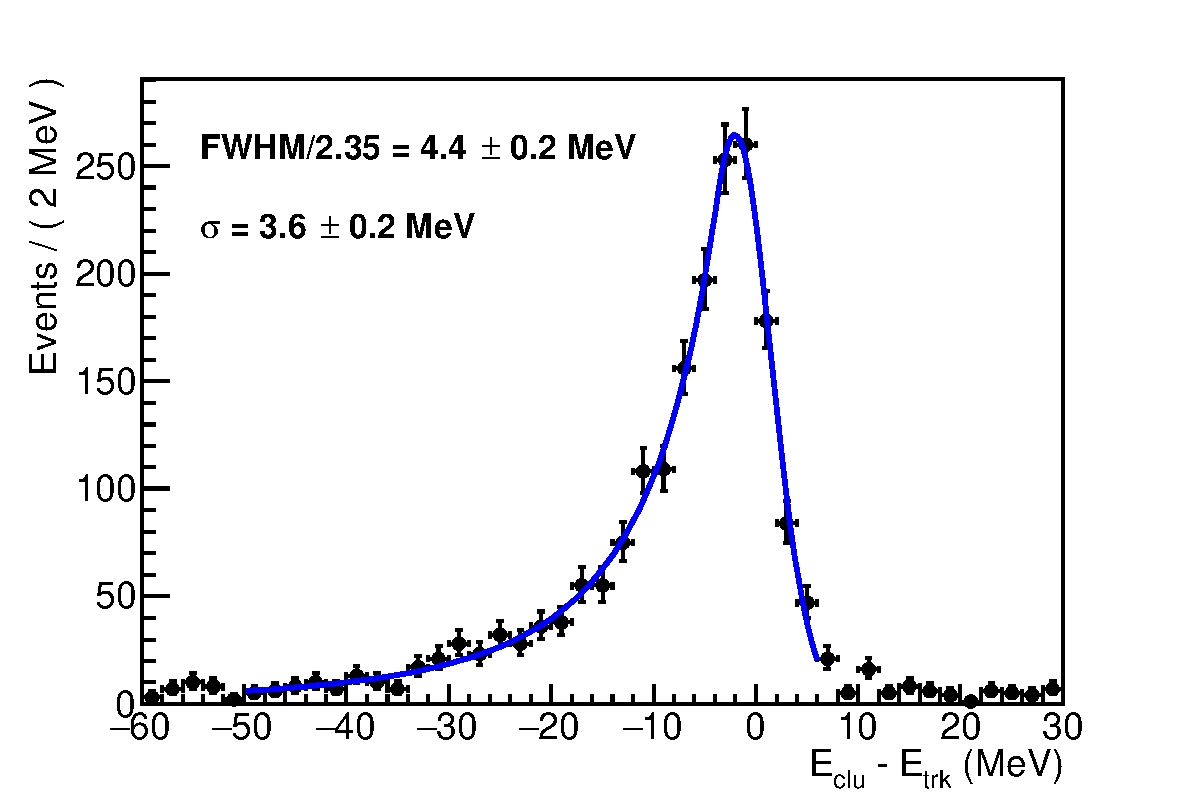
\includegraphics[width=0.45\textwidth]{Figures/baf2_1_fit.pdf} 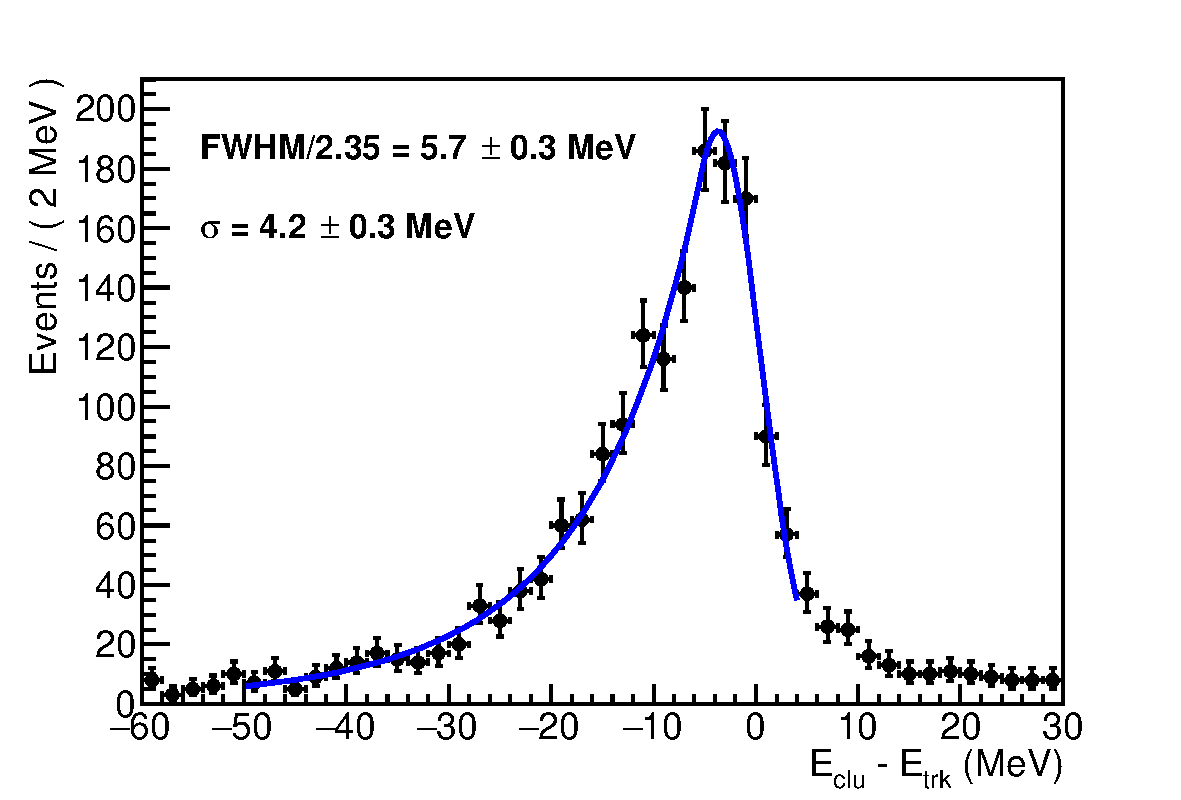
\includegraphics[width=0.45\textwidth]{Figures/csi_1_fit.pdf} 
\end{center}
\caption
{Left: Fit to the difference between the true signal electron energy and the reconstructed cluster energy, $E_{clu}-E_{trk}$, 
for $\rm BaF_2$ crystal with SL/ALD APD (simulation 1). Right: Same distribution for Csi crystal with MPPC (simulation 1).}
\label{sim::fig::fits}
\end{figure}


\begin{figure}[htb]
\begin{center}
   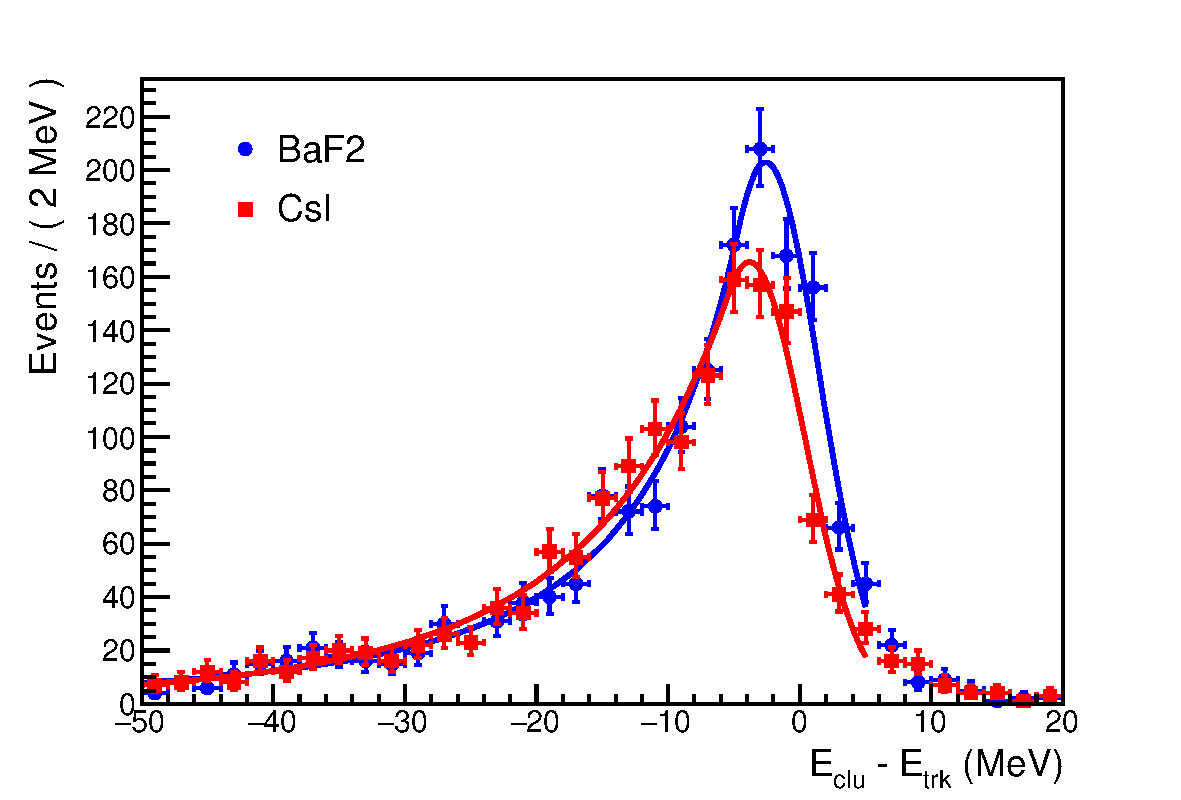
\includegraphics[width=0.7\textwidth]{Figures/compFit1.pdf}
\end{center}
\caption
{Left: Comparison of the difference between the true signal electron energy and the reconstructed cluster energy, $E_{clu}-E_{trk}$, 
for $\rm BaF_2$ with SL/ALD APD (simulation 1) and CsI with MPPC (simulation 1).}
\label{sim::fig::fitsBaCsi}
\end{figure}

\begin{figure}[htb]
\begin{center}
   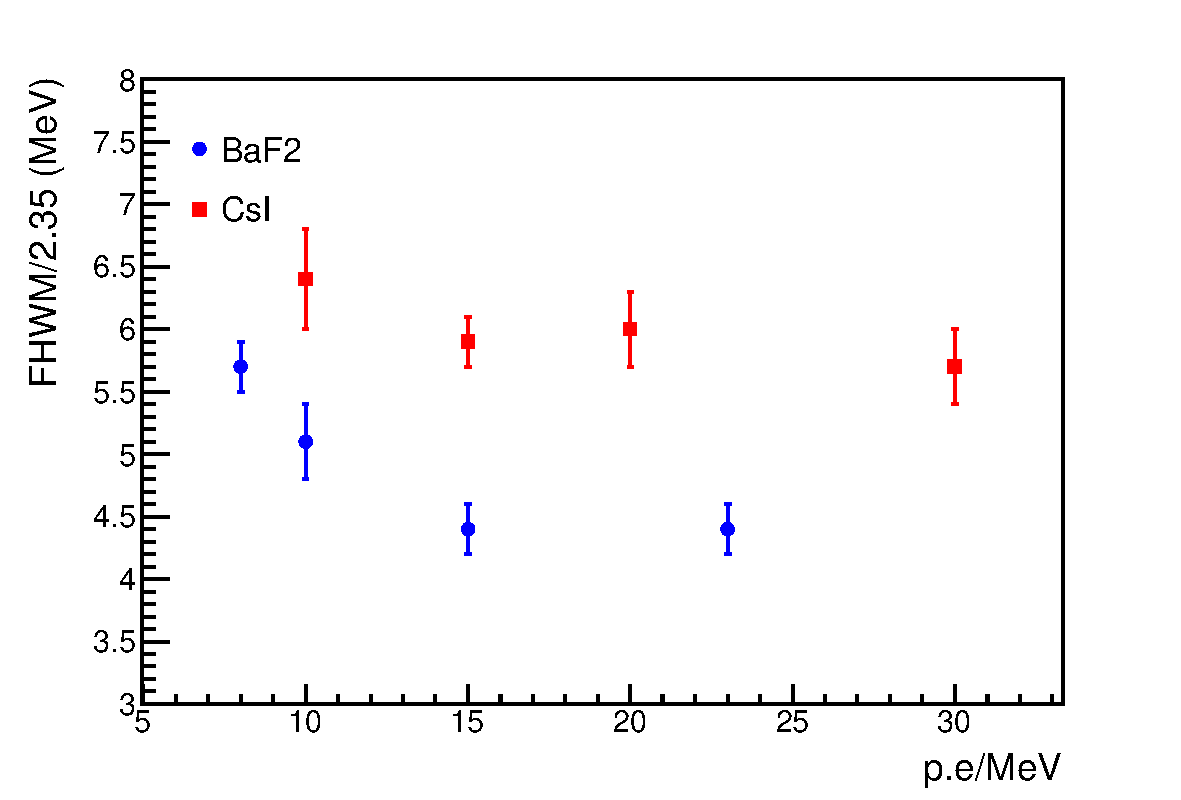
\includegraphics[width=0.45\textwidth]{Figures/npe.pdf}
   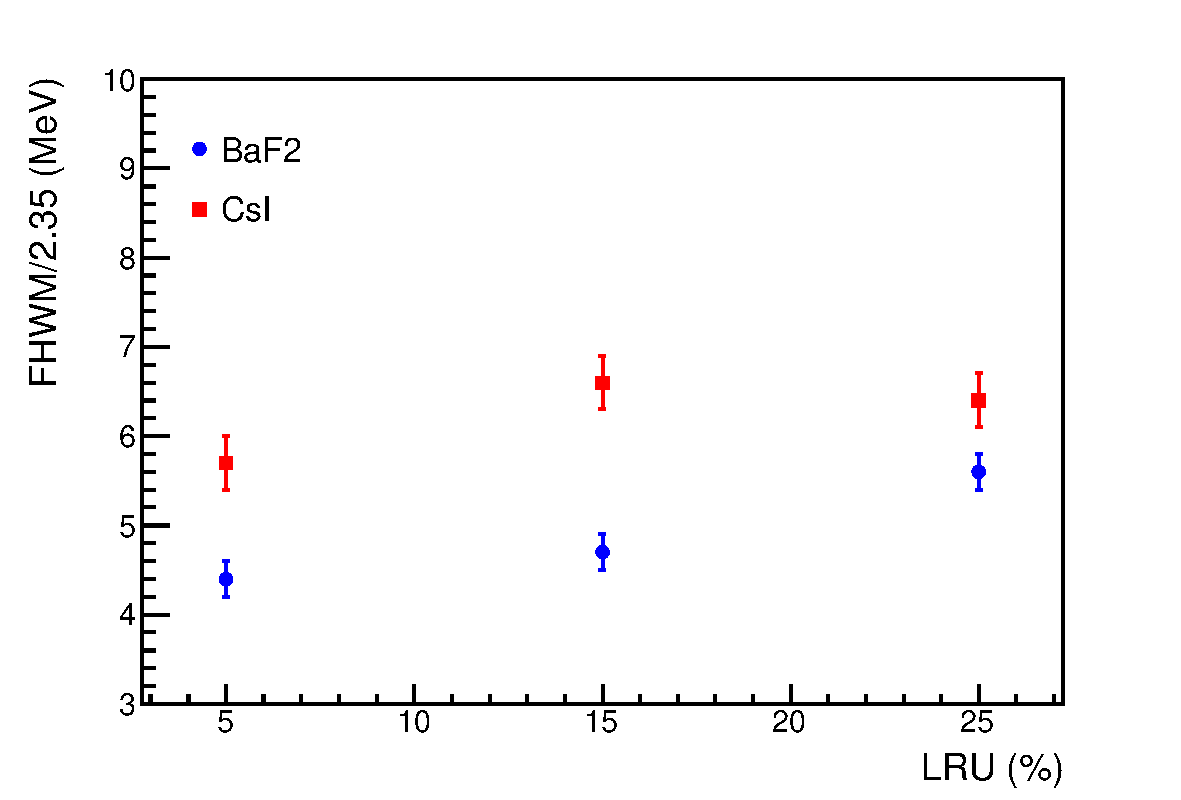
\includegraphics[width=0.45\textwidth]{Figures/lru.pdf}
\end{center}
\caption
{Left: Distribution of the FWHM/2.35 as a function of the number of p.e./MeV for $\rm BaF_2$ (red) and CsI (blue) crystals. 
Right: Distribution of the FWHM/2.35 as a function of longitudinal response uniformity (LRU) for $\rm BaF_2$ (red) and 
CsI (blue) crystals.}
\label{sim::fig::param}
\end{figure}


\begin{figure}[htb]
\begin{center}
   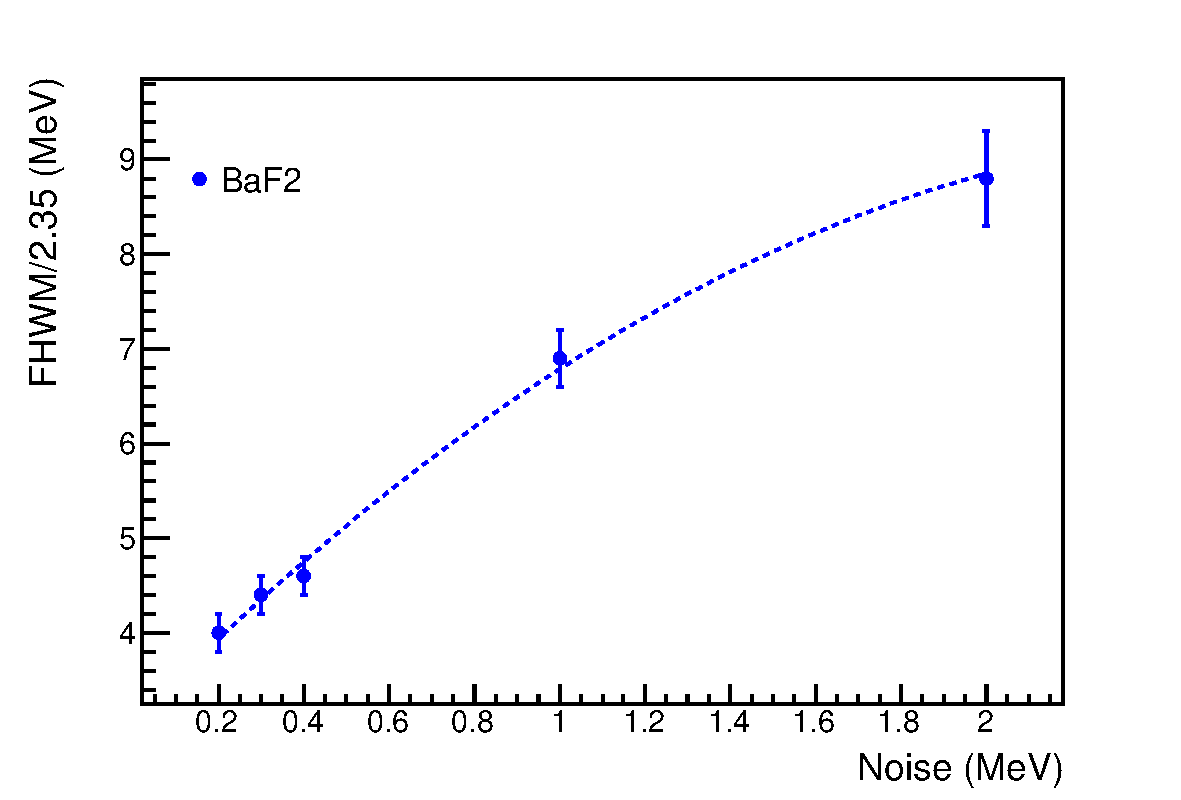
\includegraphics[width=0.7\textwidth]{Figures/noise.pdf}
\end{center}
\caption
{Distribution of the FWHM/2.35 as a function of the readout noise for $\rm BaF_2$ crystals, together with a fit using a 
second-order polynomial (dashed line). The resolution FWHM/2.35 for CsI is at the level of $\sim 6$ MeV. }
\label{sim::fig::param2}
\end{figure}



\begin{figure}[htb]
\begin{center}
   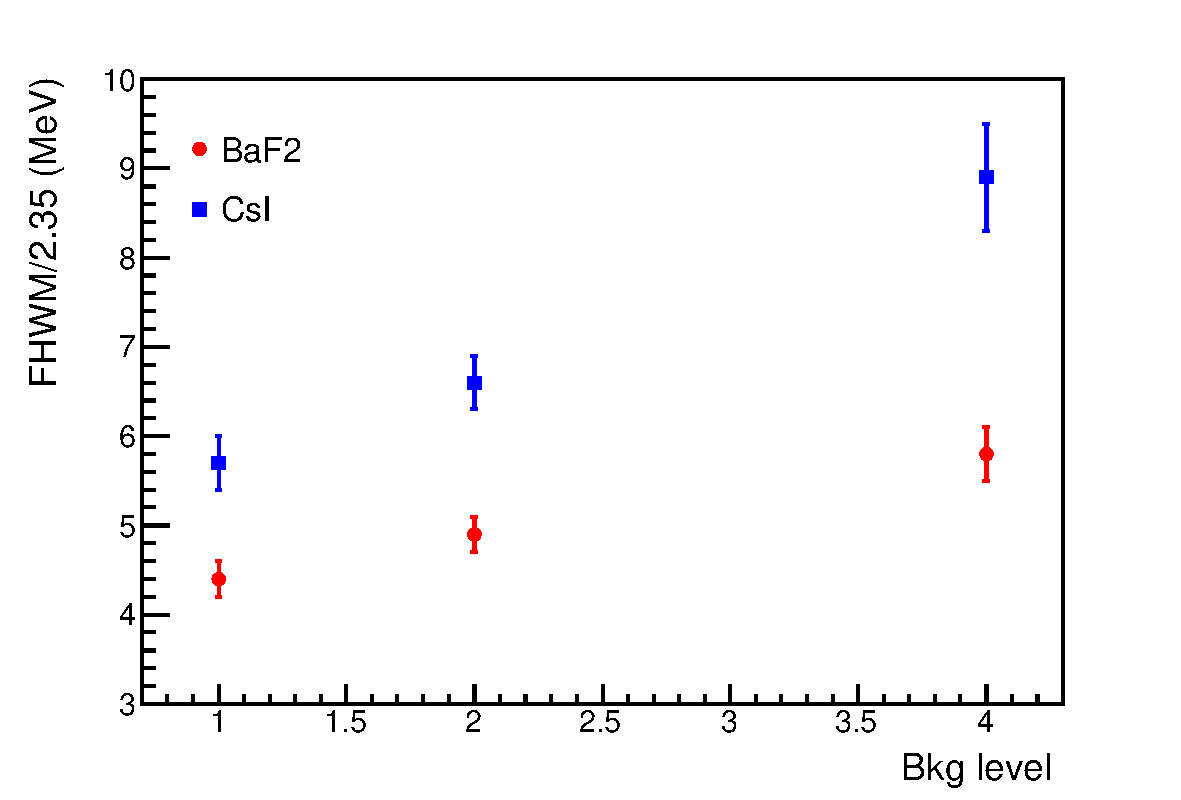
\includegraphics[width=0.7\textwidth]{Figures/bkg.pdf}
\end{center}
\caption
{Distribution of the FWHM/2.35 as a function of the background level for $\rm BaF_2$ (red) and CsI (blue) crystals.}
\label{sim::fig::bkg}
\end{figure}

\begin{figure}[htb]
\begin{center}
   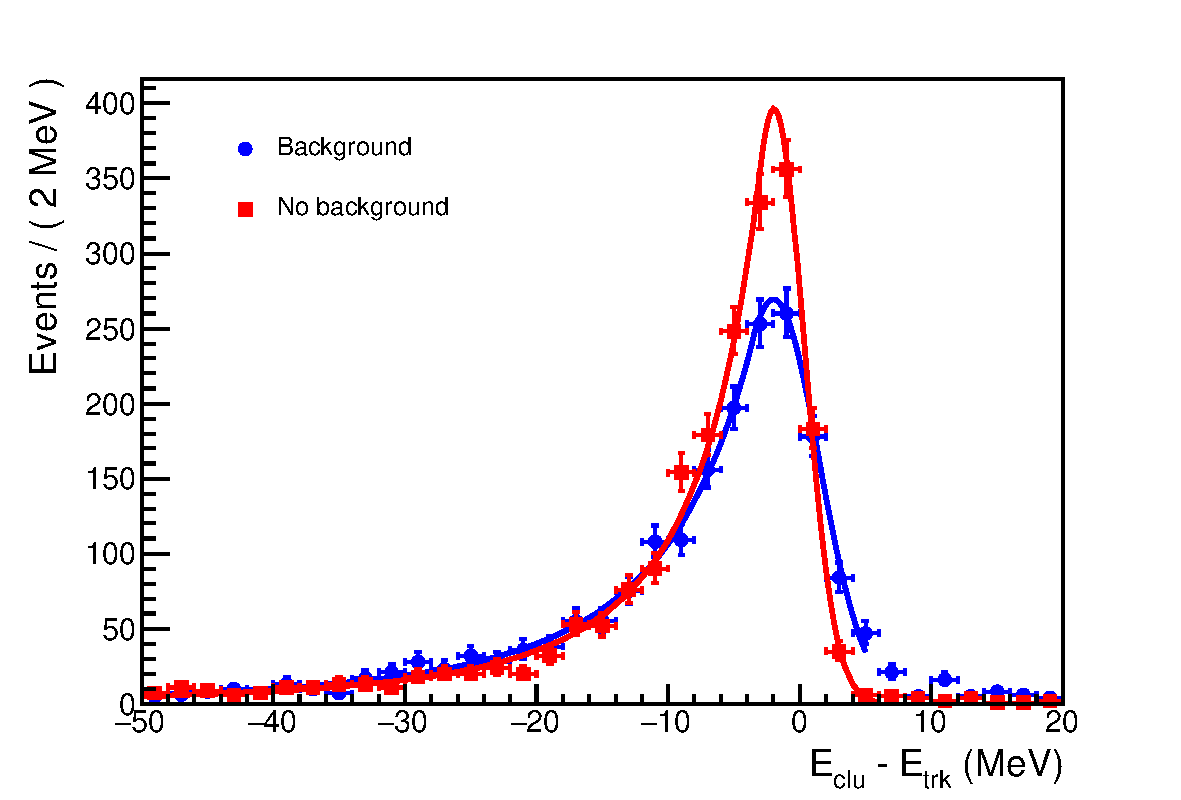
\includegraphics[width=0.28\textwidth]{Figures/compFit4.pdf} 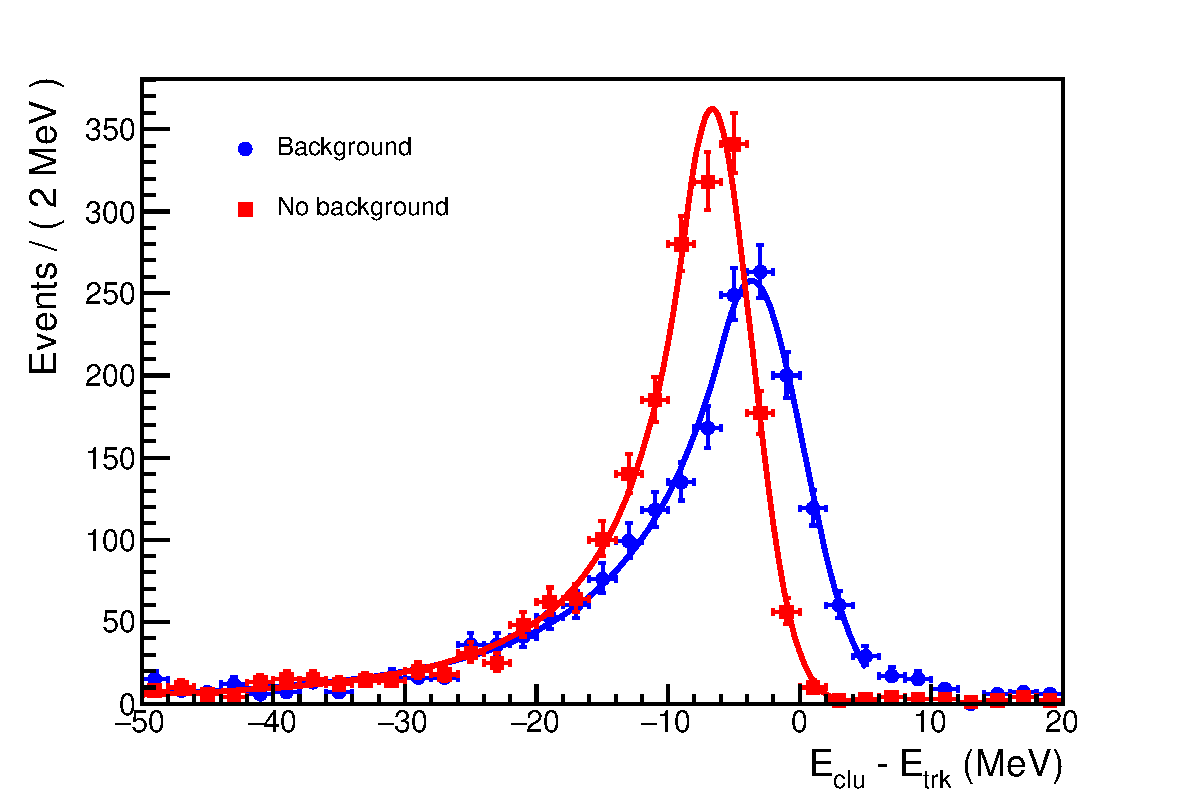
\includegraphics[width=0.28\textwidth]{Figures/compFit6.pdf}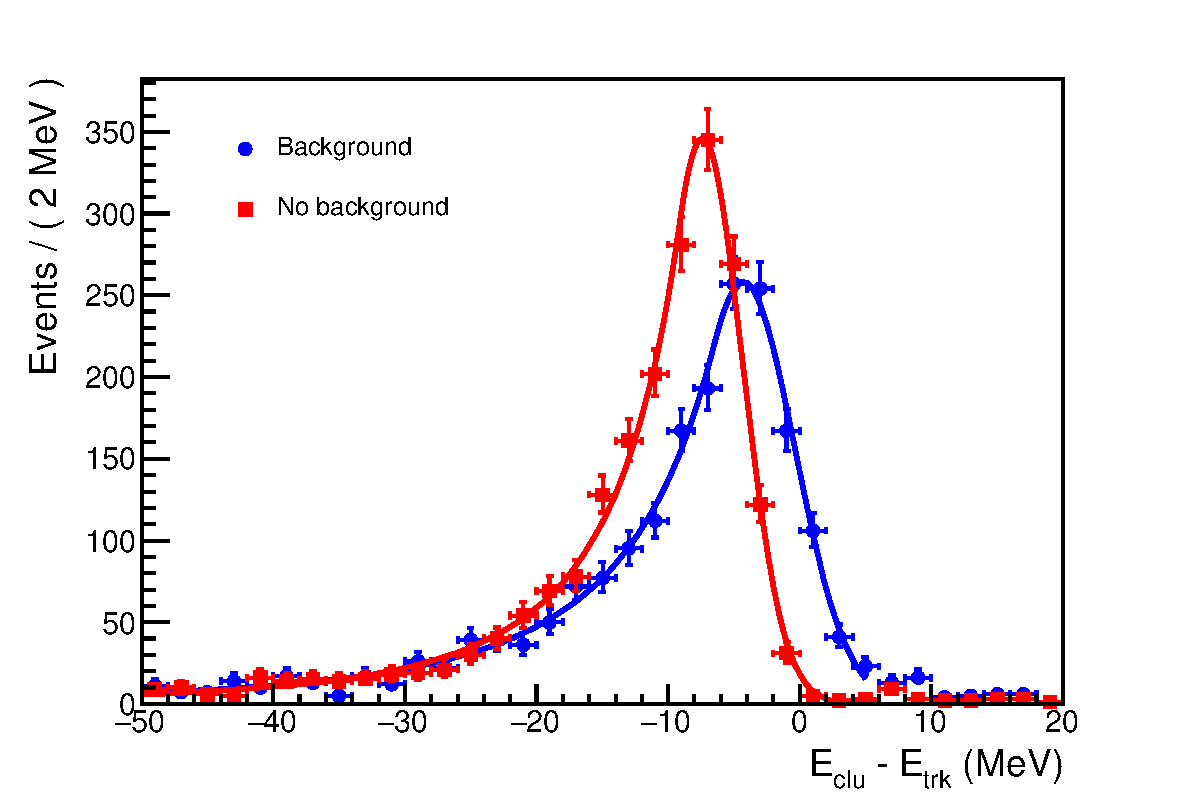
\includegraphics[width=0.28\textwidth]{Figures/compFit7.pdf}
   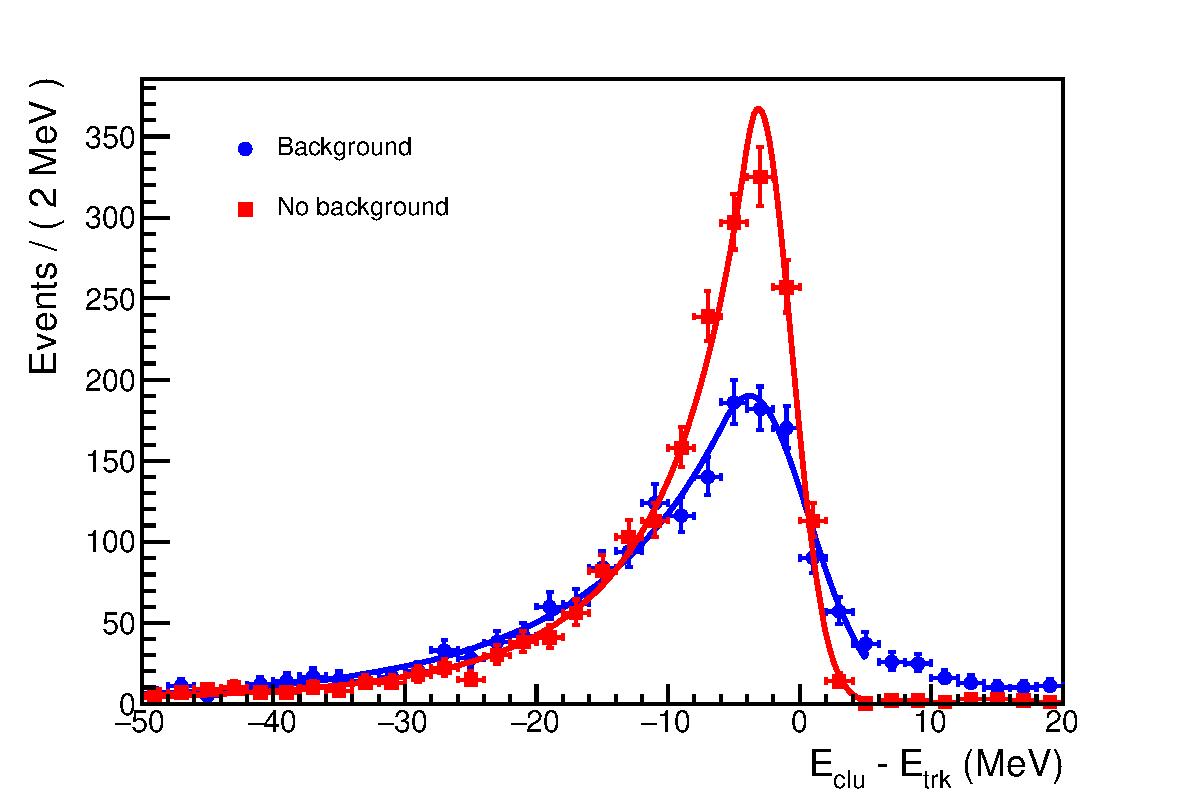
\includegraphics[width=0.28\textwidth]{Figures/compFit5.pdf} 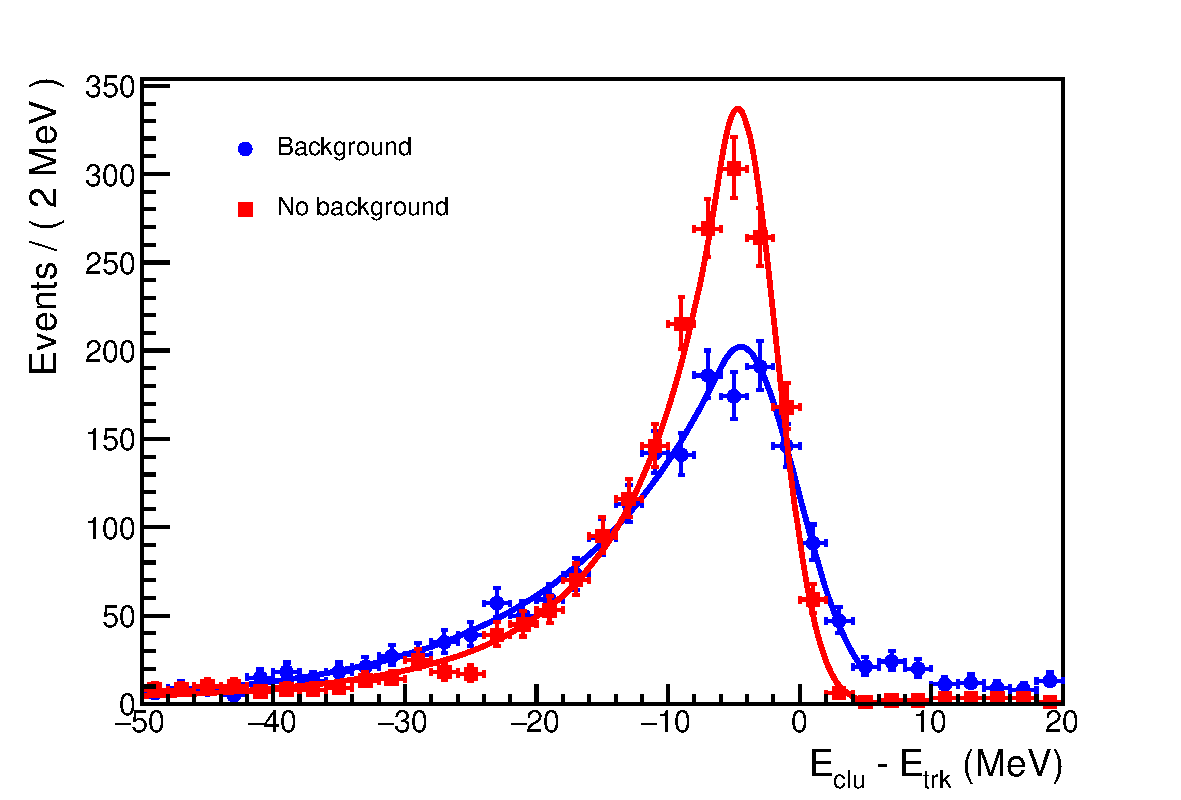
\includegraphics[width=0.28\textwidth]{Figures/compFit8.pdf}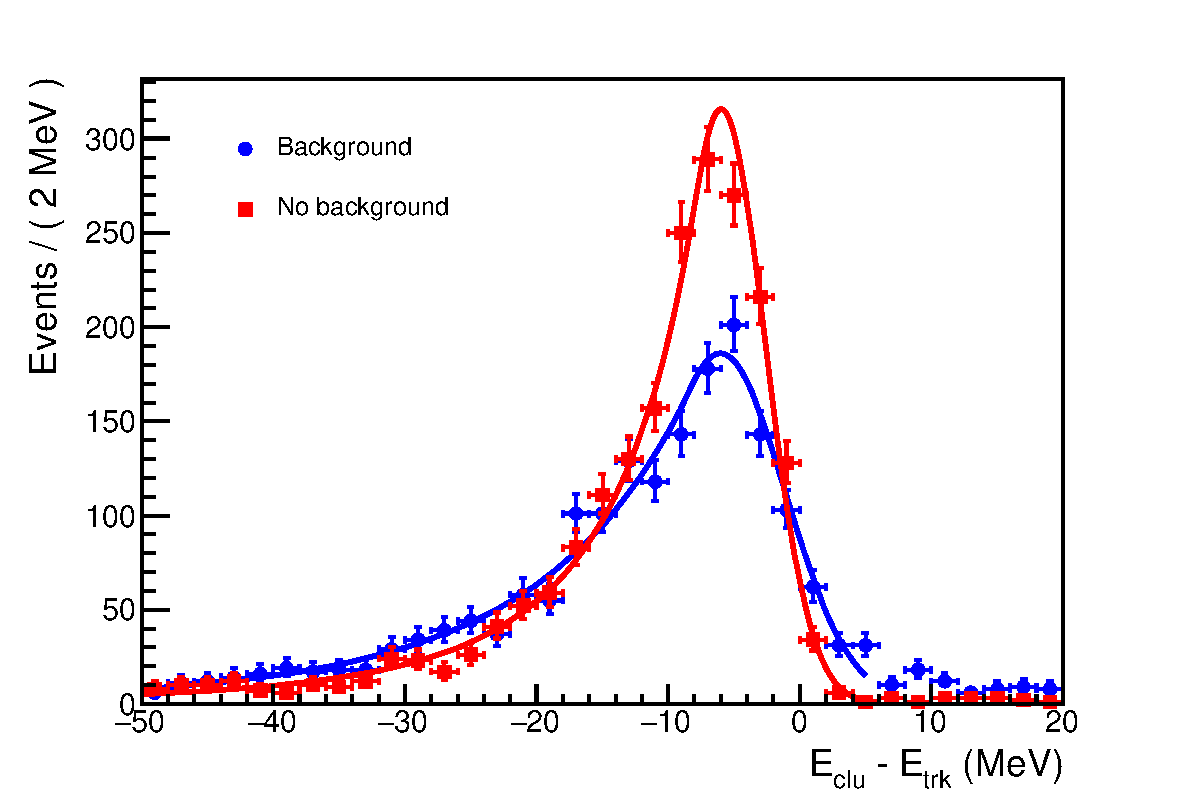
\includegraphics[width=0.28\textwidth]{Figures/compFit9.pdf}
\end{center}
\caption
{Top: Fits to the difference between the true signal electron energy and the reconstructed cluster energy, $E_{clu}-E_{trk}$, for $\rm BaF_2$ crystals 
with / without background for different values of energy cut in the clustering algorithm: 1.0 MeV (left), 1.5 MeV (middle) and 2.0 MeV (right). Bottom: Same 
distributions for CsI crystals. }
\label{sim::fig::fitsNobkg2}
\end{figure}



\begin{figure}[htb]
\begin{center}
   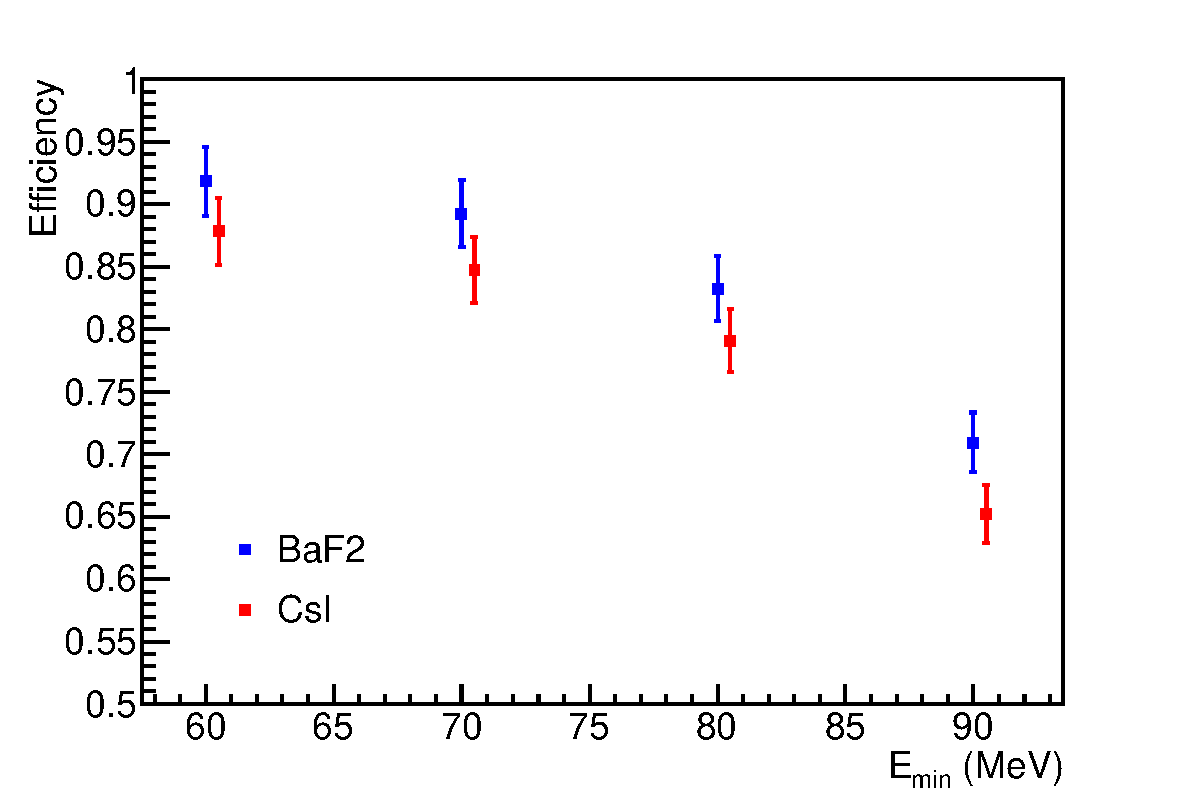
\includegraphics[width=0.7\textwidth]{Figures/effi.pdf}
\end{center}
\caption
{Efficiency as a function of the cut on the cluster energy for $\rm BaF_2$ (red) and CsI (blue) crystals. The efficiency is defined as the number of 
events having a reconstructed track and an electromagnetic cluster above a given energy threshold normalized to the number of events containing a reconstructed 
track. The peak of each cluster energy distribution is arbitrarily set to 100 MeV.}
\label{sim::fig::effi}
\end{figure}

\clearpage
